% !TEX root = ../Dokumentation.tex
\subsection{Gesamtübersicht}
\begin{figure}[H]%Position festigen
\centering
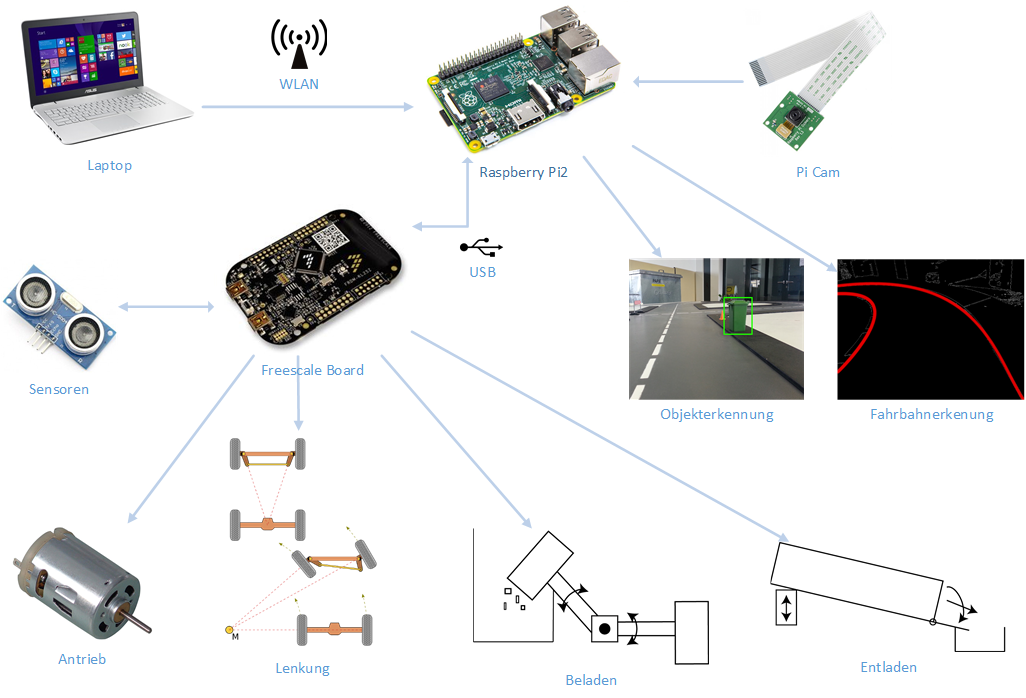
\includegraphics[width=0.9\textwidth]{03_Loesungskonzept/pictures/uebersichtszeichnung.png}
\caption{Übersichtszeichnung}
\label{fig:Übersichtszeichnung}
\end{figure}
\subsubsection{Zusammenspiel}
Wie die obige Darstellung zeigt, besteht zwischen allen Komponenten ein enges Zusammenspiel. So wird beispielsweise die gesamte Bilderkennung über den Minicomputer gesteuert. Dieser erhält seine Daten einerseits durch die Kamera, aber auch von den Sensoren welche über den Mikrocontroller an ihn gesendet werden. Nachdem die Informationen bearbeitet wurden, werden Befehle an den Mikrocontroller geschickt, welcher die Ansteuerung der Motoren übernimmt. Die Motoren wiederum, lösen die mechanischen Bewegungen aus wie z.B die Schwenkung der Kamera oder das Senken des Greifarmes.
\subsubsection{Schnittstellen}
\begin{figure}[H]%Position festigen
\centering
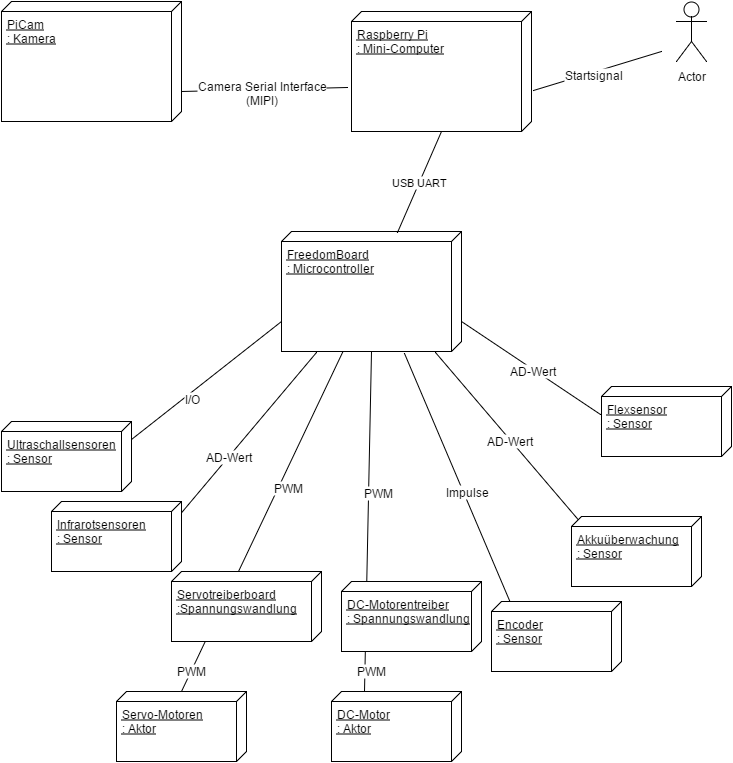
\includegraphics[width=0.9\textwidth]{03_Loesungskonzept/pictures/Verteilungsdiagramm.png}
\caption{Schnittstellenübersicht}
\label{fig:Verteilungsdiagramm}
\end{figure}\flushleft
In Abbildung \ref{fig:Verteilungsdiagramm} wird eine detaillierte Ansicht der Komponente dargestellt, insbesondere was die Schnittstellen betrifft. So ist erkennbar, dass der Mikrocontroller als Hauptknoten fungiert und als Schnittstelle für analoge wie auch digitale Signale dient.
\subsubsection{Regelkreise}
\underline{\textbf{Geschwindigkeitsregelung}}\\[0.2cm]
Damit das Fahrzeug mit einer konstanten Geschwindigkeit fahren kann, muss ein Regler eingebaut werden.
\begin{figure}[H]
	\centering
	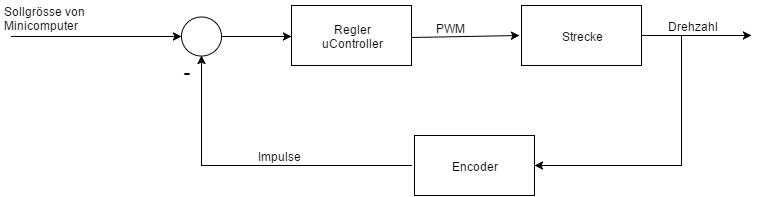
\includegraphics[width=1\textwidth]{03_Loesungskonzept/pictures/Gesch_Regelung.png}
	\label{Regelung_Gesch}
	\caption{Grober Antriebsregelkreis}
\end{figure}\flushleft
%In Abbildung \ref{Regelung_Gesch} 
Hier ist der grobe Regelkreis des Antriebs zu sehen. Der Sollwert wird vom Minicomputer vorgegeben und an das Mikrocontrollerboard weitergeleitet. In diesem wird dann die Regelung implementiert. Der Regelausgang ist ein PWM\footnote{PWM= Pulsweiten Moduliertes Signal} Signal, welches die Geschwindigkeit des Antriebsmotors bestimmt. Die Drehzahl des Antriebes wird über einen Encoder an der Antriebswelle zurück gelesen.\\[0.2cm]
\underline{\textbf{Lenkregelung}}\\[0.2cm]
Damit des Fahrzeug auf der Strecke bleiben kann, braucht es einen Regelkreis für die Steuerung. Der grobe Regelkreis ist hier aufgezeigt.
\begin{figure}[H]
	\centering
	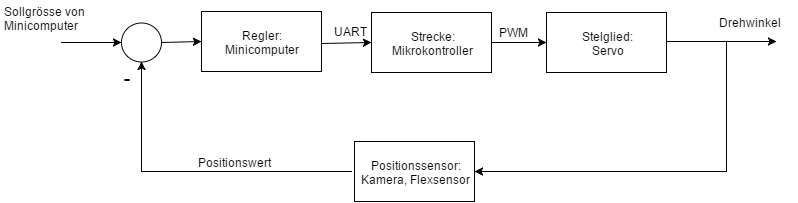
\includegraphics[width=1\textwidth]{03_Loesungskonzept/pictures/Lenk_Regelung.png}
	\label{Regelung_Lenken}
	\caption{Grober Steuerungs Regelkreis }
\end{figure}\flushleft
%Wie in Abbildung \ref{Regelung_Lenken} 
Wie hier zu sehen ist, befindet sich der Regler auf dem Minicomputer. Der Regelausgang wird über UART\footnote{UART= Serielles Kommunikationsprotokoll} auf das Mikrocontrollerboard weitergeleitet. Dieser ändert darauf hin das PWM Signal zu Servo. Die Positionsdetektion wird über die Kamera/Flexsensor realisiert. Das ist nur eine Übersicht über den Regelkreis.
